\documentclass[12pt]{article}
\usepackage{amsmath,amssymb}
\usepackage{geometry}
\usepackage{enumitem}
\usepackage{tikz}
\geometry{margin=0.8in}

\newcommand{\graphgrid}{%
\begin{center}
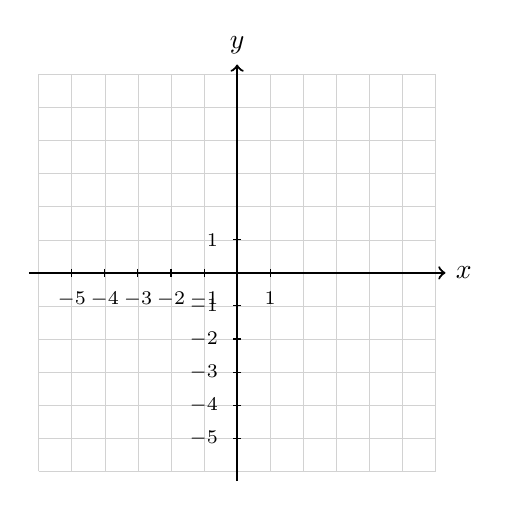
\begin{tikzpicture}[scale=0.42]
  \draw[step=1cm,gray!35,very thin] (-6,-6) grid (6,6);
  \draw[->,thick] (-6.3,0)--(6.3,0) node[right] {$x$};
  \draw[->,thick] (0,-6.3)--(0,6.3) node[above] {$y$};
  \foreach \x in {-5,...,-1,1,...,5} \draw (\x,0.12)--(\x,-0.12) node[below=2pt] {\scriptsize $\x$};
  \foreach \y in {-5,...,-1,1,...,5} \draw (0.12,\y)--(-0.12,\y) node[left=2pt] {\scriptsize $\y$};
\end{tikzpicture}
\end{center}}

\title{Algebra II Practice: Polynomials, Rational Functions, and Inequalities}
\author{}
\date{}

\begin{document}
\maketitle

\section*{Formula and Definition Sheet}

\subsection*{Polynomial Functions}
A polynomial has the form
\[
  P(x)=a_nx^n+a_{n-1}x^{n-1}+\cdots+a_1x+a_0,
  \qquad a_n\ne0.
\]
The \textbf{degree} is $n$, and $a_n$ is the \textbf{leading coefficient}. The leading term determines end behavior.

\begin{center}
\begin{tabular}{c|c|c}
Degree and leading coefficient & As $x\to-\infty$ & As $x\to\infty$\\ \hline
Even degree, $a_n>0$ & $P(x)\to\infty$ & $P(x)\to\infty$\\
Even degree, $a_n<0$ & $P(x)\to-\infty$ & $P(x)\to-\infty$\\
Odd degree, $a_n>0$ & $P(x)\to-\infty$ & $P(x)\to\infty$\\
Odd degree, $a_n<0$ & $P(x)\to\infty$ & $P(x)\to-\infty$
\end{tabular}
\end{center}

If $(x-r)^m$ is a factor, then $r$ is a zero of \textbf{multiplicity} $m$. At a zero of odd multiplicity, the graph crosses the $x$-axis; at a zero of even multiplicity, it touches and turns. Larger multiplicities flatten the graph near the zero.

\[
  \text{Remainder theorem: dividing $P(x)$ by $x-c$ leaves remainder $P(c)$.}
\]
\[
  \text{Factor theorem: $(x-c)$ is a factor exactly when $P(c)=0$.}
\]
For an integer-coefficient polynomial, possible rational zeros are
\[
  \pm\frac{\text{factor of constant term}}{\text{factor of leading coefficient}}.
\]

\subsection*{Polynomial Inequalities}
To solve $P(x)>0$, $P(x)<0$, $P(x)\ge0$, or $P(x)\le0$:
\begin{enumerate}[leftmargin=1.6em,itemsep=0.15em]
  \item Move all terms to one side and factor completely.
  \item Mark every real zero on a number line.
  \item Determine the sign on each interval. The sign changes across odd-multiplicity zeros but not across even-multiplicity zeros.
  \item Include zeros for $\le$ or $\ge$; exclude them for $<$ or $>$.
\end{enumerate}

\subsection*{Rational Functions}
A rational function is a quotient
\[
  R(x)=\frac{P(x)}{Q(x)},\qquad Q(x)\ne0.
\]
Values making the \emph{original} denominator zero are excluded from the domain.

\begin{itemize}[leftmargin=1.5em,itemsep=0.2em]
  \item A canceled denominator factor creates a \textbf{hole}. Substitute its $x$-value into the simplified function to find the hole's $y$-coordinate.
  \item An uncanceled denominator zero creates a \textbf{vertical asymptote}.
  \item $x$-intercepts come from uncanceled numerator zeros. The $y$-intercept is $R(0)$ when defined.
\end{itemize}

\subsection*{Horizontal and Oblique Asymptotes}
An asymptote describes the graph's long-run behavior; the graph may cross a horizontal or oblique asymptote.

For
\[
  R(x)=\frac{P(x)}{Q(x)},
  \qquad n=\deg P,\quad m=\deg Q,
\]
compare the degrees after common factors have been canceled:
\[
\begin{array}{c|c}
\text{Degree comparison} & \text{End-behavior asymptote}\\ \hline
n<m & y=0\\
n=m & y=\dfrac{\text{leading coefficient of }P}
                 {\text{leading coefficient of }Q}\\
n=m+1 & \text{oblique (slant) asymptote from polynomial division}
\end{array}
\]

A \textbf{horizontal asymptote} $y=L$ means
\[
  R(x)\to L \quad\text{as }x\to\infty
  \quad\text{or as }x\to-\infty.
\]
It describes end behavior, not a boundary that the graph cannot cross.

An \textbf{oblique asymptote}, also called a \textbf{slant asymptote}, is a line $y=mx+b$ approached by the graph as $x\to\pm\infty$. Use polynomial division:
\[
  \frac{P(x)}{Q(x)}=(mx+b)+\frac{\text{remainder}}{Q(x)}.
\]
If the remainder term approaches $0$, then $y=mx+b$ is the oblique asymptote. For example,
\[
  \frac{x^2+3x+5}{x-1}=x+4+\frac9{x-1},
\]
so the oblique asymptote is $y=x+4$.

If $n>m+1$, polynomial division gives a higher-degree polynomial asymptote rather than a horizontal or oblique line.

For rational inequalities, use zeros and vertical asymptotes as critical numbers. Never include a value excluded from the domain.

\clearpage
\section*{Instructions}
Complete all 20 questions in 60 minutes. For multiple-choice questions, select the best answer. For graphing questions, label intercepts, holes, and asymptotes and show correct end behavior. Give exact values and use interval notation for inequalities.

\section*{Problems}
\begin{enumerate}[leftmargin=*,itemsep=1.1em]
  \item Which statement describes the end behavior of
  \[
    f(x)=-3x^5+2x^3-7?
  \]
  \begin{enumerate}[label=\Alph*.,itemsep=0pt]
    \item Both ends rise.
    \item Both ends fall.
    \item The left end falls and the right end rises.
    \item The left end rises and the right end falls.
  \end{enumerate}

  \item What is the remainder when $2x^3-3x^2-5x+7$ is divided by $x-2$?
  \begin{enumerate}[label=\Alph*.,itemsep=0pt]
    \item $-9$ \item $-1$ \item 1 \item 9
  \end{enumerate}

  \item Which is the complete factorization of $x^3-4x^2-x+4$?
  \begin{enumerate}[label=\Alph*.,itemsep=0pt]
    \item $(x-4)(x-1)(x+1)$
    \item $(x+4)(x-1)(x+1)$
    \item $(x-4)(x^2+1)$
    \item $(x-1)^2(x-4)$
  \end{enumerate}

  \item For $P(x)=(x+2)^2(x-3)^3$, which statement is true?
  \begin{enumerate}[label=\Alph*.,itemsep=0pt]
    \item The graph crosses at both $x=-2$ and $x=3$.
    \item The graph touches at both $x=-2$ and $x=3$.
    \item The graph touches at $x=-2$ and crosses with flattening at $x=3$.
    \item The graph crosses with flattening at $x=-2$ and touches at $x=3$.
  \end{enumerate}

  \item Solve $(x-4)(x+1)(x-2)\le0$.
  \begin{enumerate}[label=\Alph*.,itemsep=0pt]
    \item $(-\infty,-1]\cup[2,4]$
    \item $[-1,2]\cup[4,\infty)$
    \item $(-\infty,-1)\cup(2,4)$
    \item $[-1,4]$
  \end{enumerate}

  \item Solve $x^4-5x^2+4>0$.
  \begin{enumerate}[label=\Alph*.,itemsep=0pt]
    \item $(-2,-1)\cup(1,2)$
    \item $(-\infty,-2)\cup(-1,1)\cup(2,\infty)$
    \item $(-\infty,-1)\cup(1,\infty)$
    \item $(-2,2)$
  \end{enumerate}

  \item Graph $y=(x+3)(x-1)^2$. Label each intercept and state the multiplicity of each zero.
  \graphgrid

  \item Graph $y=-(x+2)^2(x-2)^2$. Label each intercept and show the correct behavior at both zeros.
  \graphgrid

  \item For
  \[
    R(x)=\frac{x^2-9}{x^2-x-6},
  \]
  which statement is correct?
  \begin{enumerate}[label=\Alph*.,itemsep=0pt]
    \item There is a hole at $\left(3,\frac65\right)$ and a vertical asymptote at $x=-2$.
    \item There is a hole at $(-2,-1)$ and a vertical asymptote at $x=3$.
    \item There are vertical asymptotes at $x=-2$ and $x=3$.
    \item There is a hole at $(3,0)$ and no vertical asymptote.
  \end{enumerate}

  \item What are the vertical and horizontal asymptotes of
  \[
    R(x)=\frac{2x^2+x-3}{x^2-4}?
  \]
  \begin{enumerate}[label=\Alph*.,itemsep=0pt]
    \item $x=\pm2$ and $y=0$
    \item $x=\pm2$ and $y=2$
    \item $x=2$ and $y=2$
    \item $x=-2$ and $y=\frac12$
  \end{enumerate}

  \item What are the intercepts of
  \[
    h(x)=\frac{x-4}{x^2-x-6}?
  \]
  \begin{enumerate}[label=\Alph*.,itemsep=0pt]
    \item $x$-intercept $(4,0)$; $y$-intercept $\left(0,\frac23\right)$
    \item $x$-intercept $(-4,0)$; $y$-intercept $\left(0,-\frac23\right)$
    \item $x$-intercepts $(3,0)$ and $(-2,0)$; $y$-intercept $\left(0,\frac23\right)$
    \item No $x$-intercept; $y$-intercept $(0,4)$
  \end{enumerate}

  \item Solve
  \[
    \frac{(x-1)(x+2)}{x-3}\ge0.
  \]
  \begin{enumerate}[label=\Alph*.,itemsep=0pt]
    \item $(-\infty,-2]\cup[1,3)$
    \item $[-2,1]\cup(3,\infty)$
    \item $[-2,3)$
    \item $(-2,1)\cup[3,\infty)$
  \end{enumerate}

  \item Graph
  \[
    y=-\frac{2}{x-1}+3.
  \]
  Label both asymptotes and at least two points on the graph.
  \graphgrid

  \item Graph
  \[
    y=\frac{x^2-1}{x^2+x}.
  \]
  Label the hole, vertical asymptote, horizontal asymptote, and intercepts.
  \graphgrid

  \item If $x-2$ is a factor of $x^3+kx^2-5x+6$, what is $k$?
  \begin{enumerate}[label=\Alph*.,itemsep=0pt]
    \item $-4$ \item $-1$ \item 1 \item 4
  \end{enumerate}

  \item What is the slant asymptote of
  \[
    y=\frac{x^2+3x+5}{x-1}?
  \]
  \begin{enumerate}[label=\Alph*.,itemsep=0pt]
    \item $y=x-4$ \item $y=x+1$ \item $y=x+4$ \item $y=3x+5$
  \end{enumerate}

  \item Solve $x(x-2)^2(x+3)<0$.
  \begin{enumerate}[label=\Alph*.,itemsep=0pt]
    \item $(-\infty,-3)\cup(0,2)$
    \item $(-3,0)$
    \item $(-3,0)\cup(2,\infty)$
    \item $(-\infty,-3)\cup(0,\infty)$
  \end{enumerate}

  \item Graph
  \[
    y=-\frac12(x+1)(x-2)(x-4).
  \]
  Label all intercepts and show the correct end behavior.
  \graphgrid

  \item Graph
  \[
    y=\frac{x^2-4}{x-1}.
  \]
  Label the vertical and slant asymptotes and all intercepts.
  \graphgrid

  \item A rational function has an $x$-intercept at $x=3$, a vertical asymptote at $x=-2$, a horizontal asymptote at $y=1$, and a hole where $x=1$. Write one possible function in factored form. Then simplify it, find the hole's $y$-coordinate, and sketch its graph.
  \graphgrid
\end{enumerate}

\end{document}
